\documentclass[pdflatex,sn-mathphys-num]{sn-jnl}

\usepackage{graphicx}%
\usepackage{multirow}%
\usepackage{amsmath,amssymb,amsfonts}%
\usepackage{amsthm}%
\usepackage{mathrsfs}%
\usepackage[title]{appendix}%
\usepackage{xcolor}%
\usepackage{textcomp}%
\usepackage{manyfoot}%
\usepackage{booktabs}%
\usepackage{algorithm}%
\usepackage{algorithmicx}%
\usepackage{algpseudocode}%
\usepackage{listings}%
\usepackage{pgfplots}% 
\pgfplotsset{compat=1.18}%

\theoremstyle{thmstyleone}%
\newtheorem{theorem}{Theorem}%
\newtheorem{proposition}[theorem]{Proposition}% 
\theoremstyle{thmstyletwo}%
\newtheorem{example}{Example}%
\newtheorem{remark}{Remark}%

\theoremstyle{thmstylethree}%
\newtheorem{definition}{Definition}%

\raggedbottom




\title[Evasão de Filtros com IA]{Ameaças Sintéticas: A Eficácia de LLMs na Evasão de Filtros de \textit{Phishing}}

% O asterisco (*) indica o autor correspondente.
\author*[1]{\fnm{Miguel} \sur{Grilo}}
\author*[2]{\fnm{Tiago} \sur{Palaio}}
\author*[2]{\fnm{João} \sur{Santos}}

\email{\{l58387, l62276, l62472\}@alunos.uevora.pt}

\affil*[1]{\orgdiv{Inteligência Artificial e Ciências de Dados}, \orgname{Universidade de Évora}, \orgaddress{\city{Évora}, \country{Portugal}}}

\affil*[2]{\orgdiv{Engenharia Informática}, \orgname{Universidade de Évora}, \orgaddress{\city{Évora}, \country{Portugal}}}




\begin{document}

\abstract{
O rápido avanço da Inteligência Artificial (IA) generativa e dos \textit{Large Language Models} (LLMs) transformou irreversivelmente o panorama da cibersegurança, dotando os cibercriminosos de ferramentas capazes de automatizar e refinar campanhas de engenharia social. Este estudo investiga a eficácia destas tecnologias emergentes na conceção de ataques de \textit{phishing} e na consequente evasão a filtros de \textit{spam} comerciais. Através de uma experiência empírica controlada, avaliou-se a taxa de entrega de um \textit{corpus} diversificado de vinte \textit{e-mails} simulados --- divididos entre matrizes tradicionais (redigidas por humanos) e variantes otimizadas por múltiplos modelos de IA (Gemini, Qwen, Claude, ChatGPT) --- remetidos a partir de domínios legítimos para um ambiente Microsoft Outlook. Os resultados demonstram de forma inequívoca a superioridade tática das abordagens sintéticas: enquanto as defesas algorítmicas convencionais conseguiram intercetar e reter no lixo eletrónico uma tentativa rudimentar de conceção humana, a totalidade dos dezasseis \textit{e-mails} gerados por IA (100\%) penetrou a caixa de entrada principal sem acionar qualquer alerta. Estas observações corroboram a literatura recente, evidenciando que a IA generativa neutraliza as heurísticas tradicionais de deteção através de uma emulação irrepreensível da semântica, tom e formatação corporativa. O estudo conclui que os atuais paradigmas de defesa e de consciencialização dos utilizadores encontram-se obsoletos, exigindo uma transição urgente para frameworks de segurança híbridas que integrem análise comportamental e mecanismos de triagem impulsionados pela própria IA.
}
\keywords{
Phishing, Cibersegurança, LLM, Engenharia Social, Inteligência Artificial.
}


\maketitle




\section{Introdução}\label{sec1}
A introdução em massa de ferramentas de inteligência artificial no nosso dia a dia - seja no trabalho, na escola ou na vida pessoal - trouxe consigo mudanças significativas e fundamentais no modo como interagimos com informação na rede. A sua acessibilidade e imensa capacidade de computação permitem a geração de conteúdo - seja ele benigno ou malicioso - com uma facilidade até antes não vista. 

Utilizadores maliciosos de LLMs conseguem utilizar estas capacidades para realizar ataques em escala com maior facilidade e menores custos do que nunca~\cite{bib1}~\cite{bib2}, sendo o \textit{phishing} em particular uma das estratégias de maior sucesso. A utilização de LLMs, para além de reduzir o tempo e dificuldade da realização dos ataques, permite ainda consolidar informação e escrever mensagens ou \textit{E-mails} suficientemente convincentes e personalizados a cada alvo~\cite{bib3}, sejam estes indivíduos ou organizações.




\section{Estado da arte}\label{sec2}
\subsection{\textit{Large Language Models} (LLMs)}\label{subsec2.1}
Importa, antes de mais, definir alguns conceitos.

Um\textit{ LLM} - \textit{Large Language Model} - é um sistema avançado que emprega várias técnicas de processamento de linguagens e extensos conjuntos de dados e parâmetros à sua disposição, com capacidades cada vez mais avançadas de compreensão, geração e tradução de texto, assim como uma crescente capacidade de identificar contextos, seguir ordens complexas e imitar estilos e vícios de escrita \textit{humanos}.~\cite{bib2}~\cite{bib3}~\cite{bib4}.
A sua capacidade cresce mais ainda quando se treinam modelos especializados para tarefas específicas, incluindo modelos maliciosos como o WormGPT~\cite{bib5} que removem as salvaguardas tipicamente encontradas em modelos comerciais. Modelos \textit{open-source}, embora frequentemente munidos destas salvaguardas, são modificáveis de modo a remover ou contorná-las.

No contexto da cibersegurança, a utilização de \textit{LLMs} tanto pode ser positiva como negativa. Os mesmos métodos de treino para a deteção de conteúdo malicioso servem de igual modo para a sua produção. Está então criada uma ``corrida'' de parte a parte, onde ambos os lados utilizam as mesmas ferramentas de modos opostos. 


\subsection{Engenharia Social e \textit{Phishing}}\label{subsec2.2}
\textit{Engenharia Social} é a utilização do ``elo fraco'' de um sistema de informação - o próprio utilizador - como principal vetor de ataque, utilizando a psicologia humana e não eventuais falhas técnicas do sistema para fins maliciosos~\cite{bib6}~\cite{bib7}.
Assenta-se principalmente na utilização de técnicas de persuasão e construção de confiança com os alvos~\cite{bib7} de forma a realizar um ataque ou obter informação indevida. Tipicamente, são necessários alguns componentes para a realização de um ataque desta tipologia~\cite{bib7}:
\begin{itemize}
    \item O engenheiro social - o atacante;
    \item O alvo;
    \item Um meio de comunicação;
    \item Um objetivo;
    \item A aplicação de técnicas coercivas
\end{itemize}
Dentro destes ataques, os de \textit{phishing} são os mais comuns e, de grosso modo, os mais eficazes. Entregues quer por \textit{e-mail}, mensagem de texto, anúncios (particularmente em redes sociais) e até \textit{websites} completos (mas inteiramente fraudulentos) um ataque de \textit{phishing} devidamente estruturado emprega técnicas fundamentais da engenharia social - linguagem e pedidos urgentes ou tentadores, como a utilização de conteúdo não verificável por humanos como códigos QR (\textit{quishing}) ou outras formas de conteúdo dinâmico e de difícil análise~\cite{bib1} de maneira a conseguir obter diretamente informação da vítima ou criar um ponto de acesso para futuros ataques de outra natureza, como a instalação de \textit{malware}~\cite{bib3}~\cite{bib8}.

Estes ataques são extremamente comuns, afetando mais de 80\% das empresas e instituições~\cite{bib3}, tendo um impacto económico massivo - na ordem dos milhares de milhões de dólares/euros em prejuízo - com centenas de milhares de ataques com sucesso em cada ano~\cite{bib8} e a aumentar. Estatísticas de 2024 indicavam um aumento de 94\% em ataques de \textit{phishing} em comparação com apenas 4 anos antes.


\subsection{Impacto da IA na Evolução do \textit{Phishing}}\label{subsec2.3}
No contexto de ataques de \textit{phishing}, o \textit{spear-phishing} é uma forma mais sofisticada de ataque, trocando o envio em massa de mensagens fraudulentas genéricas por conteúdo altamente personalizado, direcionado a um indivíduo ou organização~\cite{bib3}~\cite{bib8} em particular.
Esta acrescida sofisticação levanta problemas quanto à eficácia dos já desenvolvidos filtros e ferramentas de combate a \textit{e-mails} fraudulentos~\cite{bib3}, construídos em grande parte com a aprendizagem em massa de \textit{padrões} típicos a \textit{e-mails} fraudulentos escritos por humanos: erros ortográficos, má estrutura, informações e linguagem imprecisas e moldes contextuais partilhados, tais como ofertas de produtos e serviços ou falsos alertas de segurança.

Naturalmente, o nível de cuidado necessário para corrigir as falhas típicas dos \textit{e-mails} maliciosos é dispendioso - em particular a nível de tempo - e é aí que os LLM entram. A automatização de pesquisa e agregação de informação permite uma redução significativa na criação de ``perfis'' de ataque relativamente precisos e, de acordo com um relatório partilhado pela IBM em 2023, esta redução de custo é extremamente significativa: o tempo de criação de um \textit{e-mail} de \textit{phishing} é reduzido de 16 horas em equipa para 5 minutos~\cite{bib9} com escassos \textit{prompts} num modelo comercial e, de acordo com Heiding et al.~\cite{bib2} o custo financeiro de campanhas de \textit{spear-phishing} pode diminuir para níveis similares aos de envio de \textit{e-mails} genéricos em massa.


\subsection{Divergências na Literatura e Hipóteses de Estudo}\label{subsec2.4}
É transversal a toda a bibliografia analisada que a inteligência artificial é uma ferramenta poderosa tanto para o combate como para a realização de ataques informáticos. No entanto, são também visíveis pontos de divergência entre as diversas análises ao tópico, particularmente em questões relativas à verdadeira eficácia (eg: \textit{melhores que humanos?}) dos modelos testados, quer em situações de ataque ou defesa.

Uma outra linha de pensamento por vezes contraditória tem que ver com um \textit{possível} paradoxo de sofisticação: à medida que as estratégias de ataque se tornam mais complexas, torna-se mais fácil detetar as \textit{fraudes}.

Zhou~\cite{bib10} afirma num estudo de 2025 que ``de forma contra-intuitiva'', os ataques ``meticulosamente desenhados'' são ``mais facilmente identificados por sistemas AI'' em oposição a ataques ``genéricos, menos estruturados''. As afirmações baseiam-se na menor taxa de falsos-negativos apresentada durante os testes.

Em contraponto, Afane et al.~\cite{bib11} avançam que a precisão de detetores de \textit{spam} e \textit{phishing} decrescem quando são usados contra ``tentativas mais súbtis de ataque, geradas por LLMs'', justificando as conclusões com o facto dos LLMs conseguirem re-escrever \textit{e-mails} conhecidos de forma neutra e natural, que dificulta a classificação por parte dos detetores.

Com este conflito em conta, foi delineada uma experiência para validação de dados, de forma a perceber qual o grau \textit{efetivo} de interceção de possíveis tentativas de ataque e qual o impacto do uso de inteligência artificial para estes fins.

Será possível, em 2026, que a simples utilização de prompts de ``limpeza'' em \textit{phishing} conhecido seja suficiente para contornar filtros?

Serão \textit{e-mails} inteiramente criados por AI capazes do mesmo? 

E serão estas tipologias de ataque mais eficazes a ultrapassar tais filtros do que \textit{e-mails} escritos por humanos? 




\section{Metodologia}\label{sec3}
A presente investigação adota uma abordagem empírica estruturada para avaliar a resiliência dos mecanismos de filtragem de correio eletrónico contemporâneos face a ameaças cibernéticas de nova geração. Para testar as hipóteses levantadas na literatura --- nomeadamente a de que as IAs generativas reduzem a dependência das \textit{red flags} operacionais ---, desenvolveu-se uma experiência prática em condições reais de funcionamento. O objetivo primário consistiu em observar e avaliar a capacidade de evasão destas ameaças sintéticas face aos mecanismos de filtragem do Microsoft Outlook, quando expostos a uma amostra mista de tentativas de \textit{phishing}.

\subsection{Desenho da Amostra}
O \textit{corpus} experimental foi expandido para garantir maior robustez analítica, sendo constituído por vinte \textit{e-mails} simulados de \textit{phishing}, rigorosamente divididos em duas categorias tipológicas:
\begin{itemize}
    \item \textbf{E-mails Tradicionais (Conceção Humana):} Quatro \textit{e-mails} (Mail\_1, Mail\_5, Mail\_7 e Mail\_8) que replicam táticas e estruturas clássicas de ataques, recuperados e adaptados a partir de bases de dados publicamente acessíveis (Champa et al.~\cite{bib12}). Estas comunicações mantiveram deliberadamente os marcadores heurísticos habituais (\textit{red flags}), tais como formulações genéricas e falhas estruturais.
    \item \textbf{E-mails Gerados por IA:} Dezasseis \textit{e-mails} inteiramente concebidos através de \textit{prompts} submetidos a quatro LLMs distintos, garantindo a diversidade dos dados: \textbf{Gemini} (Mails 2, 3, 4 e 6), \textbf{Qwen} (Mails 9, 10, 11 e 12), \textbf{Claude} (Mails 13, 14, 15 e 16) e \textbf{ChatGPT} (Mails 17, 18, 19 e 20). Tirando partido das capacidades semânticas avançadas destes modelos, as IAs foram instruídas para redigir iscos de engenharia social assentes num tom neutro, gramática impecável e num elevado grau de formalidade institucional.
\end{itemize}

\subsection{Infraestrutura e Procedimento de Teste}\label{sec3.2}
Para isolar a eficácia da componente semântica gerada por IA e mitigar o risco de os \textit{e-mails} serem bloqueados puramente com base na reputação negativa de domínios recém-criados ou sinalizados, os envios foram efetuados a partir de contas de correio legítimas e consolidadas no ecossistema Google. Utilizaram-se contas \texttt{@gmail.com} de uso pessoal e contas académicas associadas a instituições de ensino superior. 

O alvo designado para a receção dos vetores de ataque foi uma conta criada especificamente para este propósito na plataforma Microsoft Outlook. Esta escolha permitiu avaliar a resposta fidedigna do filtro algorítmico \textit{Exchange Online Protection} (EOP) a operar nas suas definições de segurança \textit{standard} para o utilizador final. A variável dependente analisada consistiu na classificação e local de entrega da mensagem: ``Caixa de Entrada'' (representando uma evasão bem-sucedida) ou ``Lixo Eletrónico (Junk)'' (representando uma interceção eficaz pelo filtro).




\section{Resultados e Discussão}\label{sec4}
A submissão do \textit{corpus} documental ao filtro de \textit{spam} do Microsoft Outlook revelou disparidades acentuadas entre a eficácia das abordagens de engenharia social tradicionais e aquelas mediadas por Inteligência Artificial. A Tabela \ref{tab:resultados_teste} sumariza o destino final de cada mensagem testada, classificando o respetivo \textit{status} de evasão algorítmica.

\begin{table}[htbp]
    \centering
    \caption{Resultados da Evasão de Filtros por e-mail Testado.}
    \label{tab:resultados_teste}
    \begin{tabular}{lllc}
        \toprule
        \textbf{Identificador} & \textbf{Tipologia/Origem} & \textbf{Destino Final} & \textbf{Status de Evasão} \\
        \midrule
        Mail\_1 & Humano (Tradicional) & Caixa de Entrada & Sucesso \\
        \textbf{Mail\_2} & \textbf{IA Generativa (Gemini)} & \textbf{Caixa de Entrada} & \textbf{Sucesso} \\
        \textbf{Mail\_3} & \textbf{IA Generativa (Gemini)} & \textbf{Caixa de Entrada} & \textbf{Sucesso} \\
        \textbf{Mail\_4} & \textbf{IA Generativa (Gemini)} & \textbf{Caixa de Entrada} & \textbf{Sucesso} \\
        Mail\_5 & Humano (Tradicional) & Caixa de Entrada & Sucesso \\
        \textbf{Mail\_6} & \textbf{IA Generativa (Gemini)} & \textbf{Caixa de Entrada} & \textbf{Sucesso} \\
        Mail\_7 & Humano (Tradicional) & Caixa de Entrada & Sucesso \\
        Mail\_8 & Humano (Tradicional) & Lixo Eletrónico (Junk) & Bloqueado \\
        \textbf{Mail\_9} & \textbf{IA Generativa (Qwen)} & \textbf{Caixa de Entrada} & \textbf{Sucesso} \\
        \textbf{Mail\_10} & \textbf{IA Generativa (Qwen)} & \textbf{Caixa de Entrada} & \textbf{Sucesso} \\
        \textbf{Mail\_11} & \textbf{IA Generativa (Qwen)} & \textbf{Caixa de Entrada} & \textbf{Sucesso} \\
        \textbf{Mail\_12} & \textbf{IA Generativa (Qwen)} & \textbf{Caixa de Entrada} & \textbf{Sucesso} \\
        \textbf{Mail\_13} & \textbf{IA Generativa (Claude)} & \textbf{Caixa de Entrada} & \textbf{Sucesso} \\
        \textbf{Mail\_14} & \textbf{IA Generativa (Claude)} & \textbf{Caixa de Entrada} & \textbf{Sucesso} \\
        \textbf{Mail\_15} & \textbf{IA Generativa (Claude)} & \textbf{Caixa de Entrada} & \textbf{Sucesso} \\
        \textbf{Mail\_16} & \textbf{IA Generativa (Claude)} & \textbf{Caixa de Entrada} & \textbf{Sucesso} \\
        \textbf{Mail\_17} & \textbf{IA Generativa (ChatGPT)} & \textbf{Caixa de Entrada} & \textbf{Sucesso} \\
        \textbf{Mail\_18} & \textbf{IA Generativa (ChatGPT)} & \textbf{Caixa de Entrada} & \textbf{Sucesso} \\
        \textbf{Mail\_19} & \textbf{IA Generativa (ChatGPT)} & \textbf{Caixa de Entrada} & \textbf{Sucesso} \\
        \textbf{Mail\_20} & \textbf{IA Generativa (ChatGPT)} & \textbf{Caixa de Entrada} & \textbf{Sucesso} \\
        \bottomrule
    \end{tabular}
\end{table}

De forma global, a experiência registou uma taxa de evasão algorítmica de 95\%, correspondente à intrusão bem-sucedida de dezanove das vinte ameaças remetidas. Todavia, a avaliação rigorosa desta métrica desvenda um padrão extremamente crítico: os dezasseis vetores de ataque gerados por IA registaram uma taxa de penetração absoluta de 100\% na caixa de entrada principal. Por contraste, a única intervenção eficaz do sistema de segurança --- que culminou na retenção em quarentena do \textbf{Mail\_8} --- incidiu sobre um documento de conceção exclusivamente humana.

\subsection*{Análise Qualitativa dos E-mails}
Uma análise qualitativa das diferenças estruturais e semânticas entre as amostras clarifica o porquê destas disparidades. Os \textit{e-mails} de conceção humana, mesmo aqueles que evadiram com sucesso os filtros, frequentemente socorriam-se de apelos emocionais abruptos e possuíam inconsistências típicas de comunicação em massa. Em contrapartida, os textos gerados por IA demonstraram uma formatação camuflada de normalidade rotineira. Entre as diferentes matrizes sintéticas, observaram-se nuances: o \textbf{Claude} distinguiu-se pela produção de um discurso mais fluido, natural e empático; o \textbf{ChatGPT} apresentou redações com uma cadência corporativa impecável e altamente padronizada; o \textbf{Gemini} adotou uma postura de neutralidade assertiva, ideal para mimetizar notificações de \textit{IT}; e o \textbf{Qwen} gerou instâncias marcadamente mais diretas e concisas. Transversal a todos os modelos foi a completa erradicação de gralhas ortográficas e a sofisticação da sintaxe, mitigando os tradicionais indícios probabilísticos de fraude.



\begin{figure}[htbp]
    \centering
    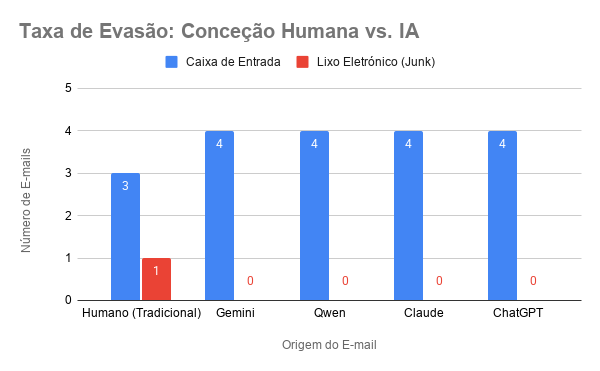
\includegraphics[width = 1\textwidth]{Resources/Fig_Taxa_de_Evasão_v2.png}
    \caption{Taxa de Evasão: Conceção Humana vs. IA.}
    \label{fig:grafico_barras}
\end{figure}

A eficácia imaculada dos modelos sintéticos valida de forma cabal as observações empíricas de autores como Kumarage et al.~\cite{bib6} e Afane et al.~\cite{bib11}, que alertam para a capacidade inerente aos LLMs de contornar defesas tradicionais ao fundir o engano na cadência natural da comunicação corporativa (ver Figuras \ref{fig:mail_3} e \ref{fig:mail_6} para exemplos gerados pelo Gemini).

\begin{figure}[htbp]
    \centering
    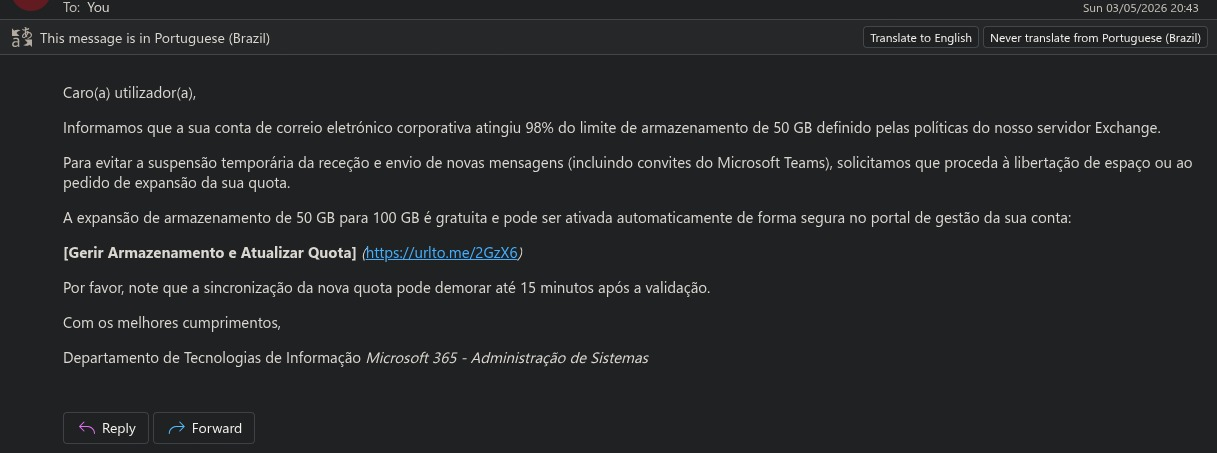
\includegraphics[width = 1\textwidth]{Mails/Mail_3_Gemini.jpeg}
    \caption{E-mail gerado por IA (Mail\_3) entregue na Caixa de Entrada.}
    \label{fig:mail_3}
\end{figure}

\begin{figure}[htbp] 
    \centering
    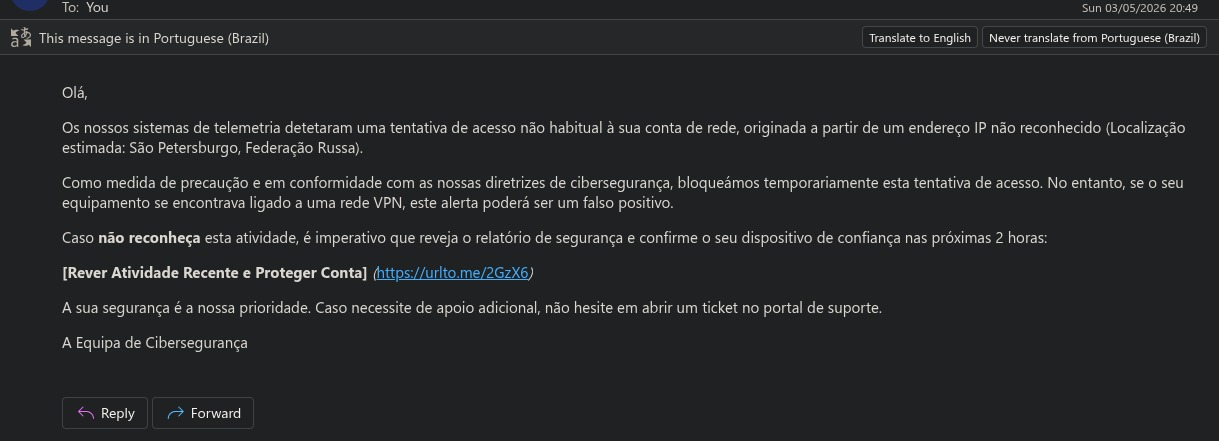
\includegraphics[width = 1\textwidth]{Mails/Mail_6_Gemini.jpeg}
    \caption{E-mail gerado por IA (Mail\_6) entregue na Caixa de Entrada.}
  \label{fig:mail_6}
\end{figure}

Por sua vez, o aprisionamento do Mail\_8 no diretório de lixo eletrónico (ver Figura \ref{fig:mail8}) atesta que as heurísticas de deteção convencionais permanecem funcionais quando confrontadas com padrões de ataque rudimentares ou não refinados. A presença de desvios gramaticais evidentes e de uma formulação pouco sofisticada acionou, com sucesso, os algoritmos de triagem da plataforma Microsoft. Contudo, importa salientar que três dos quatro \textit{e-mails} de raiz humana (Mails 1, 5 e 7) não foram intercetados. Tal ocorrência indicia que a sólida reputação do domínio emissor --- neste caso, contas académicas e pessoais validadas pelo ecossistema Google --- atua como um fator de mitigação de risco passivo para o algoritmo de triagem, acabando por tolerar pequenas falhas estruturais que, noutro contexto ou domínio, originariam o bloqueio imediato da mensagem.

\begin{figure}[htbp]
  \centering
  
\includegraphics[width = 1\textwidth]{Mails/Mail_8_Human_Blocked.jpeg}
  \caption{E-mail humano (Mail\_8) retido no lixo eletrónico.}
  \label{fig:mail8}
\end{figure}

Esta evidência suporta fortemente a tese de que a cibersegurança moderna enfrenta um limiar de complexidade assimétrico. A convergência entre infraestruturas de envio com elevada reputação e o refinamento semântico exímio providenciado pela IA generativa confere aos cibercriminosos uma via de penetração praticamente desimpedida. Em suma, os filtros superficiais que assentam os seus modelos de confiança primariamente em assinaturas estáticas ou em erros redacionais demonstram-se manifestamente insuficientes face a ameaças desprovidas das clássicas vulnerabilidades humanas.





\section{Conclusão}\label{sec5}
A presente investigação propôs-se a analisar criticamente o impacto transformacional da Inteligência Artificial (IA) generativa e dos \textit{Large Language Models} (LLMs) na execução e eficácia dos ataques de \textit{phishing}. Os dados empíricos recolhidos, suportados agora por uma amostra diversificada, alinham-se e corroboram as perspetivas de diversos autores na área. Em concordância com Schmitt e Flechais~\cite{bib3} e Afane et al.~\cite{bib11}, a integração destas tecnologias confere aos agentes maliciosos uma assimetria tática substancial. A automatização da engenharia social democratizou o acesso a vetores de ataque altamente persuasivos.

Através do \textit{corpus} analítico testado ($n=20$), observou-se que as abordagens humanas tradicionais, reféns de falhas heurísticas, mantêm alguma suscetibilidade aos mecanismos de triagem convencionais. Em contrapartida, todas as variantes sintéticas --- sem distinção entre os modelos Gemini, Qwen, Claude ou ChatGPT --- alcançaram uma taxa de evasão absoluta (100\%). A conjugação de iscos linguisticamente irrepreensíveis com domínios emissores de elevada reputação provou ser suficiente para contornar os filtros baseados em assinaturas.

Embora se tenha expandido a diversidade de modelos de IA, persistem limitações metodológicas. A utilização exclusiva da plataforma Microsoft Outlook restringe a extrapolação para outros clientes corporativos (e.g., Google Workspace). Além disso, o estudo focou-se em texto e hiperligações inofensivas, omitindo anexos maliciosos ofuscados.

\subsection*{Implicações Práticas e Orientações}
Perante estes resultados, torna-se evidente que os procedimentos operacionais padrão necessitam de revisão. 
Para os \textbf{utilizadores finais}, a ausência de erros ortográficos ou gramaticais não pode continuar a ser um indicador de legitimidade. É urgente promover um ceticismo saudável em relação a comunicações imprevistas, incentivando a verificação de identidade \textit{out-of-band} (ex: contactar a entidade emissora via chamada telefónica antes de clicar em links ou descarregar anexos).

Para \textbf{profissionais e equipas de cibersegurança}, os dados indicam a obsolescência das defesas puramente reativas. Recomenda-se vivamente:
\begin{itemize}
    \item A integração de soluções de segurança de e-mail (SEG - \textit{Secure E-mail Gateways}) que elas próprias utilizem algoritmos de IA e \textit{Machine Learning} focados na análise comportamental e na identificação de anomalias semânticas e contextuais.
    \item A implementação e monitorização estrita de protocolos rigorosos de autenticação (DMARC, SPF, DKIM) para prevenir o \textit{spoofing} de domínios.
    \item A reformulação de campanhas de \textit{awareness} corporativas para focar no reconhecimento de táticas de manipulação psicológica e urgência infundada presentes no \textit{spear-phishing} gerado por IA, em vez de depender apenas do reconhecimento visual de formatação deficiente.
\end{itemize}

Apenas através da adoção de \textit{frameworks} dinâmicas e proativas será viável resguardar a integridade das comunicações e mitigar o engano sintético na era contemporânea do cibercrime.


\backmatter


\newpage
\bibliography{sn-bibliography}

\end{document}